\begin{figure*}[t]
    \centering
    \includegraphics[width=\linewidth]{figures/fig3_zeroshot.pdf}
    \caption{\textbf{Zero-shot cross-embodiment generalization performance.} LAP-3B achieves performance comparable to the $\pi_{0.5}$-DROID on the seen embodiment. Across three previously unseen embodiments and six real-world manipulation tasks, LAP-3B attains over \textbf{50\% average zero-shot success}, delivering approximately a $2\times$ improvement over the strongest baselines, while all open-sourced VLAs collapse to zero success rate. Error bars denote 95\% finite-sample–valid confidence intervals that control the Type-I error (miscoverage) probability, following~\cite{vincent2024generalizablebehaviorcloningpolicy}.
}
    \label{fig:zero-shot}
\end{figure*}

\section{Experiments}
\label{sec:experiments}

Our experiments aim to evaluate whether language-actions provide a superior action representation for VLA pre-training. In particular, we focus on \textbf{cross-embodiment generalization}, which remains a significant limitation of state-of-the-art VLAs. Concretely, we seek to answer:
{
% \renewcommand{\theenumi}{\Alph{enumi}}
% \renewcommand{\labelenumi}{\theenumi.}
\begin{enumerate}
    \item Does LAP enable zero-shot cross-embodiment transfer?
    \item Does LAP support efficient fine-tuning to new embodiments on challenging tasks?
    \item How does LAP’s language-action representation shape the learned representations and enable strong cross-embodiment generalization?
    \item What is the effect of co-training \textsc{LAP-3B} with VQA datasets?
    \item Does LAP scale favorably with model size?
\end{enumerate}
}
To address these questions, we evaluate LAP across \textbf{four robot embodiments}, \textbf{ten real-world manipulation tasks}, and the LIBERO simulation benchmark \cite{liu2023liberobenchmarkingknowledgetransfer}. We first test out-of-the-box performance on one seen and three unseen embodiments, then study fine-tuning efficiency on new robots and tasks. We investigate the impact of LAP's language-action representation on training dynamics and conclude with an analysis of co-training with Visual--Question--Answering (VQA) datasets.

\noindent\textbf{Baselines.}
We evaluate two categories of baselines below. All replicated baselines are carefully tuned (learning rate, batch size, loss weights, etc.) for fair comparison; full details are in Appendix~\ref{app:implementation_details}.


\paragraph{Open-Sourced VLAs.}
We evaluate several publicly released VLA checkpoints to assess whether existing methods already exhibit zero-shot cross-embodiment transfer:
(1) \textbf{\bm{$\pi_{0.5}$}-DROID} \cite{intelligence2025pi05visionlanguageactionmodelopenworld}, currently the strongest VLA on the DROID benchmark;
(2) \textbf{\bm{$\pi_{0.5}$}-Base} \cite{intelligence2025pi05visionlanguageactionmodelopenworld}, the strongest publicly available VLA base model to our knowledge;
(3) \textbf{X-VLA} \cite{zheng2025xvlasoftpromptedtransformerscalable}, which explicitly targets embodiment generalization;
(4) \textbf{MolmoAct} \cite{lee2025molmoactactionreasoningmodels}; and
(5) \textbf{OpenVLA} \cite{kim2024openvlaopensourcevisionlanguageactionmodel}.


\paragraph{Action-Representation Comparison.}
To isolate the impact of language-action supervision, we train controlled baselines with identical architectures and data mixtures, differing only in action representation:

\begin{enumerate}
    \item \textbf{$\bm{\pi_{0.5}}$-replicated}: supervises the VLM using FAST tokens \cite{pertsch2025fastefficientactiontokenization}. Since the FAST tokenizer is pre-trained on substantially more robot data than our model, this forms a particularly strong baseline.
    \item \textbf{$\bm{\pi_{0}}$-replicated}: removes action supervision from the VLM entirely and only supervises the action expert, measuring the benefit of language-action pre-training.
    \item \textbf{VLA-0-replicated}: supervises the VLM following \citet{goyal2025vla0buildingstateoftheartvlas}, where continuous actions are represented as digit tokens.
\end{enumerate}
Across all experiments, we conduct \textbf{over 1300 real-robot evaluation trials}.

\subsection{Zero-Shot Cross-Embodiment Generalization}
\label{subsec:zero_shot}



\noindent\textbf{Embodiments and Tasks.}
We evaluate on four robot embodiments (Fig.~\ref{fig:zero-shot}): the DROID setup \cite{khazatsky2025droidlargescaleinthewildrobot} which is included in the pre-training mixture, three unseen embodiments---a custom 7-DoF Franka Panda robot with a novel gripper and wrist-mounted camera configuration, the 6-DoF YAM robot, and the 7-DoF Kinova robot.

We evaluate five manipulation task types (Fig.~\ref{fig:zero-shot}, top row):
\begin{enumerate}
    \item \textbf{Pick and Place}: pick up an object and place it into a container, testing generalization across gripper geometry, camera placement, and robot appearance.
    \item \textbf{Sort}: sort all objects on the table into a basket, evaluating long-horizon manipulation.
    \item \textbf{Tissue}: pull tissue from a box and place it on the table, requiring adaptive grasping of deformable objects and height reasoning.
    \item \textbf{Put Towel}: pick up a flat towel and place it into a basket, requiring precise grasp localization and large vertical motion.
    \item \textbf{Pour}: pour contents from a bowl, testing rotational control and primitive sequencing.
\end{enumerate}

These tasks require full 6-DoF manipulation, e.g., rotating the gripper to avoid collisions during sorting, and probe complementary primitive skills.

For each embodiment, we evaluate on two of these tasks with 20 trials per task. We report mean success rates with 95\% confidence intervals following the method of \cite{vincent2024generalizablebehaviorcloningpolicy}, which provides statistically valid finite-sample coverage. Unlike heuristic standard deviations, these intervals explicitly control the Type-I error (miscoverage) probability. Success metric is binary: a trial is marked successful only if the full task is completed. Results are summarized in Fig.~\ref{fig:zero-shot}.

\noindent\textbf{Seen Embodiment Evaluation.} On the in-distribution DROID setup, we observe that nearly all open-sourced VLAs fail to achieve non-trivial task success, with the sole exception of $\pi_{0.5}-\text{DROID}$ \cite{intelligence2025pi05visionlanguageactionmodelopenworld}, which has been explicitly fine-tuned on the DROID dataset \cite{khazatsky2025droidlargescaleinthewildrobot}. This highlights a critical limitation of current VLAs: despite large-scale multi-embodiment pre-training, effective deployment even on seen embodiments typically requires embodiment-specific adaptation. 

For our replicated comparison baselines, $\pi_{0.5}$-replicated and $\pi_{0}$-replicated achieve moderate and comparable performance. However, $\text{VLA-0}$-replicated consistently collapses to near-zero actions. We find this failure mode stems from overfitting to trivial predictions, which manifests as predicting only small-magnitude action tokens. This issue may be less of a concern on smaller, cleaner benchmarks such as LIBERO \cite{liu2023liberobenchmarkingknowledgetransfer} but becomes detrimental at large scale, where noise and behavioral diversity are unavoidable.

Notably, \textsc{LAP-3B} consistently outperforms $\pi_{0.5}$-replicated and $\pi_{0}$-replicated by approximately 15 percentage points across tasks, despite sharing the same backbone architecture and training data; this highlights the superiority of the language-action representation. Moreover, \textsc{LAP-3B} achieves performance on par with $\pi_{0.5}$-DROID---without any embodiment-specific fine-tuning on the DROID dataset itself. This indicates that language-action supervision enables effective learning from large-scale, heterogeneous robot data, leading to strong in-distribution performance.


\noindent\textbf{Unseen Embodiment Evaluation.} We next evaluate zero-shot transfer to three previously unseen robot embodiments. Across all settings, \textsc{LAP-3B} demonstrates a substantial and consistent advantage, with an \emph{average success rate exceeding 50\%}, representing an approximate \textbf{2$\times$ improvement over the strongest baseline}. Importantly, \textsc{LAP-3B} is the only model to achieve consistently high performance across all novel embodiments.

In contrast, all open-sourced VLAs, including $\pi_{0.5}$-DROID, which performed strongly in-distribution, fail to generate meaningful behavior on unseen robots. This sharp collapse suggests that existing VLA training recipes remain tightly coupled to embodiment-specific control conventions, preventing transfer even when visual and task semantics remain similar.


By contrast, \textsc{LAP-3B} exhibits both \emph{semantically grounded movements} and \emph{fine-grained spatial control} across embodiments. We hypothesize that the language-action interface provides a shared, embodiment-agnostic abstraction that better preserves the VLM’s generalizable visual-semantic representations while enabling precise execution under novel robot kinematics. This decoupling allows \textsc{LAP-3B} to retain coherent task intent while avoiding the embodiment-specific overfitting that hampers existing VLAs.

\begin{figure*}[t]
    \centering
    \includegraphics[width=\linewidth]{figures/fig4_finetune.pdf}
    \caption{\textbf{Fine-tuning efficiency in simulation (LIBERO) and real-world manipulation tasks}. Across both domains, \textsc{LAP-3B} adapts substantially faster than baseline policies, reaching high performance with significantly fewer epochs and demonstrations. In simulation, \textsc{LAP-3B} converges to near-optimal success within a fraction of the training steps required by baselines. On real robots, \textsc{LAP-3B} achieves comparable task performance using approximately \textbf{$\bm{2.5\times}$ fewer demonstrations}, demonstrating substantially improved data and compute efficiency when transferring to new embodiments.}
    \label{fig:libero-fine-tuning}
\end{figure*}
\vspace{2pt}

\subsection{Fine-Tuning Efficiency on New Embodiments}
\label{sec:finetuing}

While \textsc{LAP-3B} exhibits non-trivial zero-shot performance on novel embodiments for simple tasks, more challenging manipulation scenarios still require embodiment-specific adaptation at the current training scale. We therefore investigate whether LAP improves \emph{fine-tuning efficiency} along two axes: \emph{data efficiency}---requiring fewer demonstrations to reach a given performance level, and \emph{compute efficiency}---converging with fewer gradient steps.

\noindent\textbf{Simulation Fine-Tuning Experiments.}
We first fine-tune \textsc{LAP-3B} on the LIBERO simulation benchmark \cite{liu2023liberobenchmarkingknowledgetransfer} and compare against $\pi_{0.5}$-replicated and $\pi_0$-replicated baselines trained on the same pre-training mixture. We additionally report an oracle baseline, $\pi_{0.5}$-Oracle, initialized from the original $\pi_{0.5}$ weights pre-trained on substantially larger datasets.


As shown in Fig.~\ref{fig:libero-fine-tuning}(a), \textsc{LAP-3B} converges substantially faster than all baselines. With only a single epoch of fine-tuning, \textsc{LAP-3B} already reaches 78\% success, and achieves near-maximum performance (96.8\%) within six epochs---significantly fewer updates than both replicated baselines and the oracle model \cite{intelligence2025pi05visionlanguageactionmodelopenworld}. While $\pi_{0.5}$-Oracle eventually attains slightly higher asymptotic performance after extended training, \textsc{LAP-3B} demonstrates markedly superior compute efficiency. These results indicate that language-action pre-training yields a more transferable initialization that adapts rapidly to new embodiments. We summarize LIBERO benchmark results for \textsc{LAP-3B} and baseline methods in Appendix~\ref{app:additional_results}.
% Table~\ref{tab:libero_results_small}, along with several open-source models. For a full comparison with additional open-source models, see Appendix~\ref{app:additional_results}.

\noindent\textbf{Real-World Fine-Tuning Experiments.}
We next fine-tune on two challenging real-robot tasks (Fig.~\ref{fig:libero-fine-tuning} top row, right):
\begin{itemize}
    \item \textbf{Hang Tape on Rack}: pick up the tape by its edge and hang it on the top rack, requiring dexterity and precision. The task is evaluated on the YAM robot.
    \item \textbf{Fold Towel and Place in Basket}: fold the towel in half from left to right, then place the folded towel into a basket, requiring both fine-grained dexterity and long-horizon manipulation. The task is evaluated on the Custom Franka robot.
\end{itemize}
Results are shown in Fig.~\ref{fig:libero-fine-tuning}. We evaluate task progress metrics over 20 trials per data point (see Appendix~\ref{app:evaluation_details} for details).

Across both tasks, \textsc{LAP-3B} achieves strong performance with substantially fewer demonstrations. On YAM, \textsc{LAP-3B} reaches approximately 50\% task progress using only 20 demonstrations---roughly \textbf{$\bm{2.5\times}$ demos fewer than baselines}. On Franka, \textsc{LAP-3B} consistently outperforms $\pi_{0.5}$-replicated and $\pi_0$-replicated across all data regimes. Together, these results demonstrate that language-action pre-training produces a more adaptable VLA, improving both sample efficiency and fine-tuning speed when transferring to new embodiments and tasks.


\begin{figure*}[t]
    \centering
    \includegraphics[width=\linewidth]{figures/fig5_analysis.pdf}
    \caption{
    \textbf{(a) T-SNE visualizations of learned embodiment representations} for \textsc{LAP-3B} and $\pi_{0.5}$-replicated. \textsc{LAP-3B} exhibits substantial overlap between training and unseen embodiments, whereas $\pi_{0.5}$-replicated shows limited alignment, indicating that \textsc{LAP-3B} learns more transferable, embodiment-agnostic control representations.
    \textbf{(b) Action prediction error on unseen embodiments during pre-training.} \textsc{LAP-3B} achieves consistently lower action prediction error on held-out unseen embodiments throughout training, compared to $\pi_{0.5}$-replicated and $\pi_{0}$-replicated baselines. This indicates that language-action supervision enables the model to learn control representations that generalize across embodiments, allowing more accurate action prediction on novel robots as well as smoother training dynamics.
    }
    \label{fig:analysis}
\end{figure*}

\subsection{Analyzing LAP’s Cross-Embodiment Generalization}

\noindent\textbf{T-SNE visualization of embodiment representations.}
We visualize learned embodiment features using t-SNE in Fig.~\ref{fig:analysis}(a) by embedding the average prelogits of action tokens, which capture internal control representations across robot embodiments. \textsc{LAP-3B} exhibits substantially improved alignment between unseen embodiments and training data, with features from unseen embodiments overlapping closely with those from training embodiments rather than forming separate clusters. In this representation space, stronger overlap between training and unseen embodiments indicates that the model has learned more transferable, embodiment-agnostic representations, helping explain why language-action pre-training enables strong zero-shot embodiment transfer.


\noindent\textbf{Low action prediction error on unseen embodiments.}
We next evaluate the quality of representations learned during pre-training by measuring action prediction error on held-out datasets from \emph{unseen} robot embodiments described in Sec.~\ref{sec:finetuing}. Prediction error is measured as the $\ell_2$ distance between predicted and ground-truth actions.

As shown in Fig.~\ref{fig:analysis}(b), \textsc{LAP-3B} consistently achieves lower action prediction error on unseen embodiments than baselines trained with alternative action representations, indicating that language-action supervision leads to more generalizable control representations across embodiment shifts. In addition, the prediction error decreases smoothly and monotonically over training, suggesting that LAP enables more stable training dynamics.

\begin{wraptable}{r}{0.5\columnwidth}
\vspace{-12pt}
\centering
\scriptsize
\setlength{\tabcolsep}{2pt}
\renewcommand{\arraystretch}{0.95}
\caption{Best prediction errors on held-out datasets from \emph{unseen robot embodiments} for \textsc{LAP-3B} and baseline methods. Best per row is bolded.}
\label{tab:val_losses}
\begin{tabular}{lccc}
\toprule
 & \textbf{\textsc{LAP-3B}} & $\pi_{0.5}$-replicated & $\pi_{0}$-replicated \\
\midrule
Prediction Error (Unseen) & \textbf{0.151} & 0.168 & 0.189 \\
Validation Loss (Unseen) & \textbf{0.049} & 0.051 & 0.052 \\
\bottomrule
\end{tabular}
\vspace{-12pt}
\end{wraptable}

We additionally report the best validation loss of the (flow-matching) action expert in Table~\ref{tab:val_losses}. Taken together, these results suggest that language-action pre-training does not merely stabilize optimization, but fundamentally improves how control representations transfer across embodiments—allowing \textsc{LAP-3B} to predict more accurate actions on unseen robots and explaining both its strong zero-shot performance and superior fine-tuning efficiency.





\subsection{Co-Training with Vision-Language Datasets}
\begin{wrapfigure}{r}{0.3\linewidth}
   \centering
   \vspace{-0.7cm}
  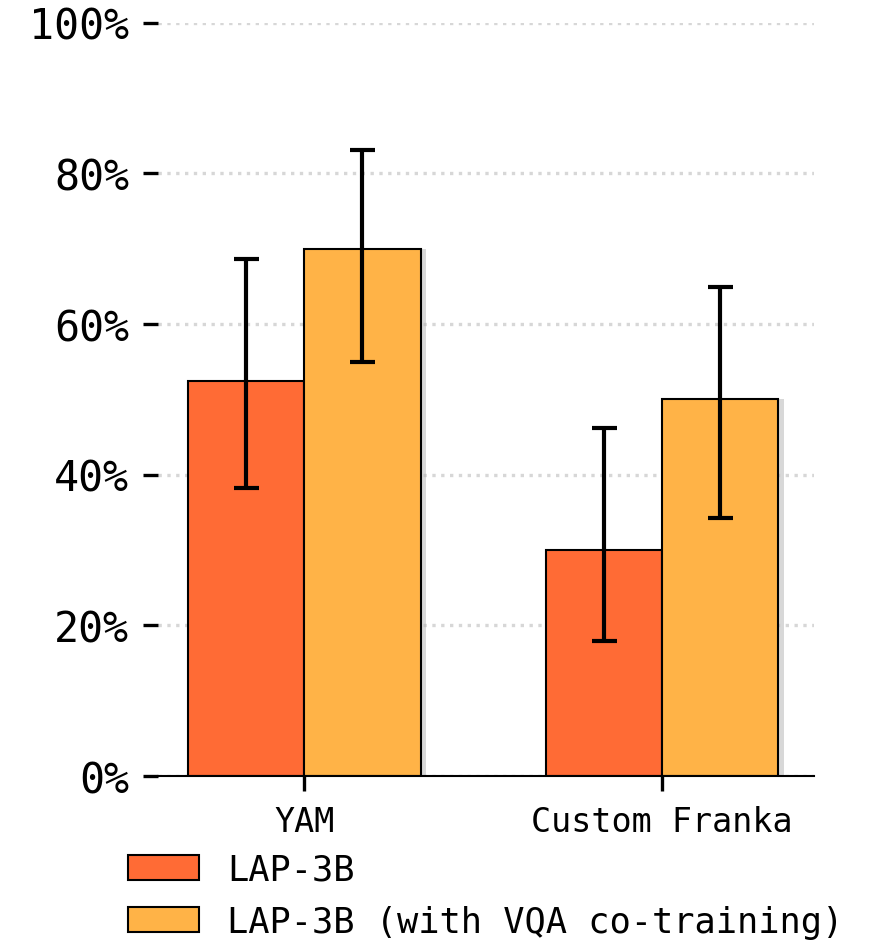
\includegraphics[width=\linewidth]{figures/fig8_cotrain.png}
  \caption{\textbf{VQA co-training} with a motion-prediction task improves cross-embodiment performance.}
  \label{fig:cotrain}
  \vspace{-0.5cm}
\end{wrapfigure}
We further investigate whether co-training with additional Visual-Question-Answering (VQA) tasks benefits \textsc{LAP-3B}.
We consider a motion-prediction task in which the model is prompted with two consecutive images and asked to predict the corresponding language-action describing the change between frames, analogous to an ``inverse dynamics'' prediction (Fig.~\ref{fig:teaser}, bottom left).
This co-training objective naturally bridges standard VQA-style supervision and our language-action prediction by sharing a unified, language-based output format.

We evaluate the resulting models on two embodiments, Custom Franka and YAM, with results shown in Fig.~\ref{fig:cotrain}.
Incorporating this motion-prediction VQA task leads to more precise action generation and improved spatial generalization, yielding higher success rates across embodiments.
In addition, co-training produces checkpoints that are easier to adapt to new tasks, enabling faster fine-tuning with fewer gradient steps and achieving higher final convergence performance (see Appendix~\ref{app:additional_results}).



\subsection{Scaling with Model Size}
% \par\medskip
\begin{wrapfigure}{r}{0.5\linewidth}
    \centering
    % \vspace{-1\baselineskip}
    \vspace{-0.4cm}
    \includegraphics[width=\linewidth]{figures/fig7_modelscaling.pdf}
    \caption{\textbf{Model scaling behavior of LAP compared to $\bm{\pi_{0.5}}$-replicated.}
    Left: Token validation loss, reported as percentage drop relative to the 4B model.
    Right: Continuous action validation loss of the diffusion-based action expert.
    \textsc{LAP-3B} improves consistently with scale, whereas the baseline saturates and degrades.}
    \label{fig:model-scaling}
    % \vspace{-20pt}
\end{wrapfigure}

We next investigate whether LAP benefits from increased model capacity, and whether its advantages persist in the large-model regime.

Using Gemma3 \cite{gemmateam2025gemma3technicalreport} as the VLM backbone, we train LAP models at 4B, 12B, and 27B parameter scales, and compare them against corresponding $\pi_{0.5}$-replicated variants, which represent the current state of the art in VLAs.

We evaluate two metrics on a held-out split comprising 2.5\% of the full data mixture: (i) token validation loss of the VLM backbone, and (ii) validation loss of the flow-matching-based action expert. For token validation loss, we report the percentage reduction relative to the 4B model, as absolute loss values are not directly comparable across different action representations. 

As shown in Fig.~\ref{fig:model-scaling}, LAP consistently attains lower validation loss across all model sizes and exhibits favorable scaling behavior, with performance improving monotonically as model capacity increases. In contrast, the $\pi_{0.5}$-replicated baseline shows early saturation and even degradation at larger scales. These results indicate that language-action supervision remains effective in the large-model regime and increasingly benefits from additional representational capacity.



